\documentclass[12pt, titlepage]{article}

\usepackage{amsmath, mathtools}
\usepackage{fullpage}
\usepackage[round]{natbib}
\usepackage{multirow}
\usepackage{booktabs}
\usepackage{tabularx}
\usepackage{graphicx}
\usepackage{float}
\usepackage{hyperref}
\usepackage{xr}
\externaldocument{../../SRS/SRS} 
\hypersetup{
	colorlinks,
	citecolor=black,
	filecolor=black,
	linkcolor=red,
	urlcolor=blue
}
\newcommand{\rref}[1]{R\ref{#1}}
\newcommand{\ddref}[1]{DD\ref{#1}}
%% Comments

\usepackage{color}

\newif\ifcomments\commentstrue

\ifcomments
\newcommand{\authornote}[3]{\textcolor{#1}{[#3 ---#2]}}
\newcommand{\todo}[1]{\textcolor{red}{[TODO: #1]}}
\else
\newcommand{\authornote}[3]{}
\newcommand{\todo}[1]{}
\fi

\newcommand{\wss}[1]{\authornote{blue}{SS}{#1}}
\newcommand{\an}[1]{\authornote{magenta}{Author}{#1}}


\newcounter{acnum}
\newcommand{\actheacnum}{AC\theacnum}
\newcommand{\acref}[1]{AC\ref{#1}}

\newcounter{ucnum}
\newcommand{\uctheucnum}{UC\theucnum}
\newcommand{\uref}[1]{UC\ref{#1}}

\newcounter{mnum}
\newcommand{\mthemnum}{M\themnum}
\newcommand{\mref}[1]{M\ref{#1}}

\begin{document}
	
	\title{Module Guide: Breaking Effect} 
	\author{Marshall Xiaoye Ma}
	\date{\today}
	
	\maketitle
	
	\pagenumbering{roman}
	
	\section{Revision History}
	
	\begin{tabularx}{\textwidth}{p{3cm}p{2cm}X}
		\toprule {\bf Date} & {\bf Version} & {\bf Notes}\\
		\midrule
		2017-10-29 & 1.0 & New document\\
		\bottomrule
	\end{tabularx}
	
	\newpage
	
	\tableofcontents
	
	\listoftables
	
	\listoffigures
	
	\newpage
	
	\pagenumbering{arabic}
	
	\section{Introduction}
	
	Decomposing a system into modules is a commonly accepted approach to developing
	software.  A module is a work assignment for a programmer or programming
	team~\citep{ParnasEtAl1984}.  We advocate a decomposition
	based on the principle of information hiding~\citep{Parnas1972a}.  This
	principle supports design for change, because the ``secrets'' that each module
	hides represent likely future changes.  Design for change is valuable in SC,
	where modifications are frequent, especially during initial development as the
	solution space is explored.  
	
	Our design follows the rules layed out by \citet{ParnasEtAl1984}, as follows:
	
	\begin{itemize}
		\item System details that are likely to change independently should be the
		secrets of separate modules.
		\item Each data structure is used in only one module.
		\item Any other program that requires information stored in a module's data
		structures must obtain it by calling access programs belonging to that module.
	\end{itemize}
	
	After completing the first stage of the design, the Software Requirements
	Specification (SRS), the Module Guide (MG) is developed~\citep{ParnasEtAl1984}. The MG
	specifies the modular structure of the system and is intended to allow both
	designers and maintainers to easily identify the parts of the software.  The
	potential readers of this document are as follows:
	
	\begin{itemize}
		\item New project members: This document can be a guide for a new project member
		to easily understand the overall structure and quickly find the
		relevant modules they are searching for.
		\item Maintainers: The hierarchical structure of the module guide improves the
		maintainers' understanding when they need to make changes to the system. It is
		important for a maintainer to update the relevant sections of the document
		after changes have been made.
		\item Designers: Once the module guide has been written, it can be used to
		check for consistency, feasibility and flexibility. Designers can verify the
		system in various ways, such as consistency among modules, feasibility of the
		decomposition, and flexibility of the design.
	\end{itemize}
	
	The rest of the document is organized as follows. Section
	\ref{SecChange} lists the anticipated and unlikely changes of the software
	requirements. Section \ref{SecMH} summarizes the module decomposition that
	was constructed according to the likely changes. Section \ref{SecConnection}
	specifies the connections between the software requirements and the
	modules. Section \ref{SecMD} gives a detailed description of the
	modules. Section \ref{SecTM} includes two traceability matrices. One checks
	the completeness of the design against the requirements provided in the SRS. The
	other shows the relation between anticipated changes and the modules. Section
	\ref{SecUse} describes the use relation between modules.
	
	\section{Anticipated and Unlikely Changes} \label{SecChange}
	
	This section lists possible changes to the system. According to the likeliness
	of the change, the possible changes are classified into two
	categories. Anticipated changes are listed in Section \ref{SecAchange}, and
	unlikely changes are listed in Section \ref{SecUchange}.
	
	\subsection{Anticipated Changes} \label{SecAchange}
	
	Anticipated changes are the source of the information that is to be hidden
	inside the modules. Ideally, changing one of the anticipated changes will only
	require changing the one module that hides the associated decision. The approach
	adapted here is called design for
	change.
	
	\begin{description}
		\item[\refstepcounter{acnum} \actheacnum \label{acHardware}:] The specific
		hardware on which the software is running.
		\item[\refstepcounter{acnum} \actheacnum \label{acInput}:] The format of the
		initial input data.
		\item[\refstepcounter{acnum} \actheacnum \label{acPO}:] If all pieces have the same initial speed after explosion.
		\item[\refstepcounter{acnum} \actheacnum \label{acPI}:] Initial component on each piece when it is generated. \an{such as texture and script.}
		\item[\refstepcounter{acnum} \actheacnum
		\label{acMove}:] The method to check if a piece is stopped. \an{In unity, negative speed means having speed towards opposite direction that is not equivalent with stop.}
		\item[\refstepcounter{acnum} \actheacnum \label{acTO}:] Different types of target object. 
		\item[\refstepcounter{acnum} \actheacnum \label{acCD}:] Method to detect if a piece is on the ground.
		\item[\refstepcounter{acnum} \actheacnum \label{acCC}:] Method to control camera.
	\end{description}
	
	\wss{There should be more than 3 anticipated changes.  Each of the leaf modules
		should map to an anticipated change.}
	\an{Add necessary anticipated changes for each leaf modules}
	\subsection{Unlikely Changes} \label{SecUchange}
	
	The module design should be as general as possible. However, a general system is
	more complex. Sometimes this complexity is not necessary. Fixing some design
	decisions at the system architecture stage can simplify the software design. If
	these decision should later need to be changed, then many parts of the design
	will potentially need to be modified. Hence, it is not intended that these
	decisions will be changed.
	
	\begin{description}
		\item[\refstepcounter{ucnum} \uctheucnum \label{ucIO}:] Input/Output devices
		(Input: Keyboard, Output: Screen).
		\item[\refstepcounter{ucnum} \uctheucnum \label{ucInput}:] There will always be
		a source of input data external to the software.
		\item[\refstepcounter{ucnum} \uctheucnum \label{ucFri}:] Input more than one coefficient of friction on the ground.
		\item[\refstepcounter{ucnum} \uctheucnum \label{ucU}:] Run this program on other platform that is different from Unity3D.
	\end{description}
	
	\wss{Is Unity an unlikely change?  I cannot remember whether this was a
		constraint in your SRS.  A more generic design is better, where the physics
		engine is a likely change and the design is done to support this change.  In
		this case there should be an anticipated change related to the change in
		physics engine.}\\
	\an{Actually on platform Unity3D is a system constraint in SRS. Add an unlikely change for this. However I believe the method I calculate displacement as well as some algorithms can be implemented on some other platforms as well.}
	\section{Module Hierarchy} \label{SecMH}
	
	This section provides an overview of the module design. Modules are summarized
	in a hierarchy decomposed by secrets in Table \ref{TblMH}. The modules listed
	below, which are leaves in the hierarchy tree, are the modules that will
	actually be implemented.
	
	\begin{description}
		\item [\refstepcounter{mnum} \mthemnum \label{mHH}:] Hardware-Hiding Module
		\item [\refstepcounter{mnum} \mthemnum \label{mBH}:] Behaviour-Hiding Module
		\item [\refstepcounter{mnum} \mthemnum \label{mIF}:] Input Module
		\item [\refstepcounter{mnum} \mthemnum \label{mPO}:] Piece Object Module
		\item [\refstepcounter{mnum} \mthemnum \label{mOGC}:] Pieces initialization module
		\item [\refstepcounter{mnum} \mthemnum \label{mDC1}:] Displacement calculation Module
		\item [\refstepcounter{mnum} \mthemnum \label{mSD}:] Software Decision Module
		\item [\refstepcounter{mnum} \mthemnum \label{mTO}:] Target Object Module
		\item [\refstepcounter{mnum} \mthemnum \label{mOC}:] Collision with ground detection Module
		\item [\refstepcounter{mnum} \mthemnum \label{mOM}:] Output Module
	\end{description}
	
	
	\begin{table}[h!]
		\centering
		\begin{tabular}{p{0.3\textwidth} p{0.6\textwidth}}
			\toprule
			\textbf{Level 1} & \textbf{Level 2}\\
			\midrule
			
			{Hardware-Hiding Module} & ~ \\
			\midrule
			
			\multirow{7}{0.3\textwidth}{Behaviour-Hiding Module} & Input Module\\			
			& Piece Object Module\\
			& Pieces initialization module\\
			& Displacement calculation module\\
			\midrule
			
			\multirow{3}{0.3\textwidth}{Software Decision Module} & Target Object Module\\
			& Collision with ground detection Module\\
			& Output Module\\
			\bottomrule
			
		\end{tabular}
		\caption{Module Hierarchy}
		\label{TblMH}
	\end{table}
	
	\wss{I would think that your physics engine would be within the software
		decision hiding modules.  You might be splitting the physics module up into
		multiple modules.  If that is the case, shouldn't there be more modules?
		Aren't there other services from Unity that you need?}\\
	\an{I only needs collision detection of unity's physics engine. In addition it is only for collision between piece and ground because collision between pieces is ignored. Other functions from unity's physics engine are turned off.}
	\section{Connection Between Requirements and Design} \label{SecConnection}
	
	The design of the system is intended to satisfy the requirements developed in
	the SRS. In this stage, the system is decomposed into modules. The connection
	between requirements and modules is listed in Table \ref{TblRT}.
	
	\section{Module Decomposition} \label{SecMD}
	
	Modules are decomposed according to the principle of ``information hiding''
	proposed by \citet{ParnasEtAl1984}. The \emph{Secrets} field in a module
	decomposition is a brief statement of the design decision hidden by the
	module. The \emph{Services} field specifies \emph{what} the module will do
	without documenting \emph{how} to do it. For each module, a suggestion for the
	implementing software is given under the \emph{Implemented By} title. If the
	entry is \emph{OS}, this means that the module is provided by the operating
	system or by standard programming language libraries.  Also indicate if the
	module will be implemented specifically for the software.
	
	Only the leaf modules in the
	hierarchy have to be implemented. If a dash (\emph{--}) is shown, this means
	that the module is not a leaf and will not have to be implemented. Whether or
	not this module is implemented depends on the programming language
	selected.
	
	\subsection{Hardware Hiding Modules (\mref{mHH})}
	
	\begin{description}
		\item[Secrets:]The data structure and algorithm used to implement the virtual
		hardware.
		\item[Services:]Serves as a hardware abstraction used by the rest of the
		system. This module provides the interface between the hardware and the
		software. So, the system can use it to display outputs or to accept inputs.
		\item[Implemented By:] OS
	\end{description}
	
	\subsection{Behaviour-Hiding Module(\mref{mBH})}
	
	\begin{description}
		\item[Secrets:]The contents of the required behaviours.
		\item[Services:]Includes programs that provide externally visible behaviour of
		the system as specified in the software requirements specification (SRS)
		documents. This module serves as a communication layer between the
		hardware-hiding module and the software decision module. The programs in this
		module will need to change if there are changes in the SRS.
		\item[Implemented By:] Breaking Effect
	\end{description}
	
	\subsubsection{Input Module (\mref{mIF})}
	
	\begin{description}
		\item[Secrets:]The format, verification of input data.
		\item[Services:]Converts the valid input data into the data structure used by other modules. \wss{You don't have an input parameters
			module.  What module will actually have its state changed?}\\
		\an{Yes I merge 2 modules for input into one module.}
		\item[Implemented By:] Breaking Effect and Unity3d. \an{GUI for input is provided by Unity3d.}
	\end{description}
	
	\subsubsection{Piece Object Module (\mref{mPO})}
	
	\begin{description}
		\item[Secrets:]Definition of class for piece object.
		\item[Services:]Define a custom class to store piece object that has much more properties and functions than game object class provided by platform. \wss{The
			difference between target and piece objects is not clear.}\\
		\an{Modify description. And I put target object module under software decision module part. Because target object is an instance of game object class provied by Unity3d while piece object is a custom class defined by myself.}
		\item[Implemented By:] Breaking Effect
	\end{description}
	
	\subsubsection{Pieces initialization module (\mref{mOGC})}
	\wss{sometimes you forget to add a space before your bracket (}\\ 
	\an{Fixed. Thank you for this remind !}
	\begin{description}
		\item[Secrets:]Preparation before explosion happens that how to generate pieces object in program.
		\item[Services:]Do traversal to initialize all pieces.
		\item[Implemented By:] Breaking Effect
	\end{description}

	\subsubsection{Displacement calculation module (\mref{mDC1})}
	
	\begin{description}
		\item[Secrets:]How the displacement are calculated.\wss{You
			cannot have the same secret in two different module.}\\
		\an{Now I consider it is unnecessary to keep two modules for displacement calculation so I merge them into one.}
		\item[Services:]Calculate trace of motion for each piece.
		\item[Implemented By:] Breaking Effect
	\end{description}
	
	\subsection{Software Decision Module(\mref{mSD})}
	
	\begin{description}
		\item[Secrets:] The design decision based on mathematical theorems, physical
		facts, or programming considerations. The secrets of this module are
		\emph{not} described in the SRS.
		\item[Services:] Includes data structure and algorithms used in the system that
		do not provide direct interaction with the user. 
		% Changes in these modules are more likely to be motivated by a desire to
		% improve performance than by externally imposed changes.
		\item[Implemented By:] Breaking Effect
	\end{description}
	
	\subsubsection{Target Object Module (\mref{mTO})}
	
	\begin{description}
		\item[Secrets:]Definition of class for target object.
		\item[Services:]It is an existing object class provided by platform for target object. 
		\item[Implemented By:] Unity3D
	\end{description}
	
	\subsubsection{Collision with ground detection Module (\mref{mOC})}
	
	\begin{description}
		\item[Secrets:] How to judge if a piece object already reaches the ground.
		\item[Services:] Detect if there is a collision between one piece and the ground. If so, set onGround value to true. 
		% Changes in these modules are more likely to be motivated by a desire to
		% improve performance than by externally imposed changes.
		\item[Implemented By:] Unity3D
	\end{description}
	
	\subsubsection{Output Module (\mref{mOM})}
	
	\begin{description}
		\item[Secrets:] Interact with platform to convert data into visualization.
		\item[Services:] Display motion of pieces in vision. Provide free camera for people to control view.
		% Changes in these modules are more likely to be motivated by a desire to
		% improve performance than by externally imposed changes.
		\item[Implemented By:] Unity3D
		\end{description}
	
	\section{Traceability Matrix} \label{SecTM}
	
	This section shows two traceability matrices: between the modules and the
	requirements and between the modules and the anticipated changes.
	
	% the table should use mref, the requirements should be named, use something
	% like fref
	\begin{table}[H]
		\centering
		\begin{tabular}{p{0.2\textwidth} p{0.6\textwidth}}
			\toprule
			\textbf{Req.} & \textbf{Modules}\\
			\midrule
			\rref{R_Inputs} & \mref{mHH},\mref{mIF}\\
			\rref{R_InitialSpeed} & \mref{mIF}\\
			\rref{R_VerifyOutput} & \mref{mIF}\\
			\rref{R_Piece} & \mref{mOGC},\mref{mOC}\\
			\rref{R_Calculate} & \mref{mAC}\\
			\rref{R_Output1} & \mref{mDC1}\\
			\rref{R_Output2} & \mref{mDC2}\\
			\bottomrule
		\end{tabular}
		\caption{Trace Between Requirements and Modules}
		\label{TblRT}
	\end{table}
	
	\begin{table}[H]
		\centering
		\begin{tabular}{p{0.2\textwidth} p{0.6\textwidth}}
			\toprule
			\textbf{AC} & \textbf{Modules}\\
			\midrule
			\acref{acHardware} & \mref{mHH}\\
			\acref{acInput} & \mref{mIF}\\
			\acref{acCF} & \mref{mOC}\\
			\bottomrule
		\end{tabular}
		\caption{Trace Between Anticipated Changes and Modules}
		\label{TblACT}
	\end{table}
	
	\section{Use Hierarchy Between Modules} \label{SecUse}
	
	In this section, the uses hierarchy between modules is
	provided. \citet{Parnas1978} said of two programs A and B that A {\em uses} B if
	correct execution of B may be necessary for A to complete the task described in
	its specification. That is, A {\em uses} B if there exist situations in which
	the correct functioning of A depends upon the availability of a correct
	implementation of B.  Figure \ref{FigUH} illustrates the use relation between
	the modules. It can be seen that the graph is a directed acyclic graph
	(DAG). Each level of the hierarchy offers a testable and usable subset of the
	system, and modules in the higher level of the hierarchy are essentially simpler
	because they use modules from the lower levels.
	
	\begin{figure}[H]
		\centering
		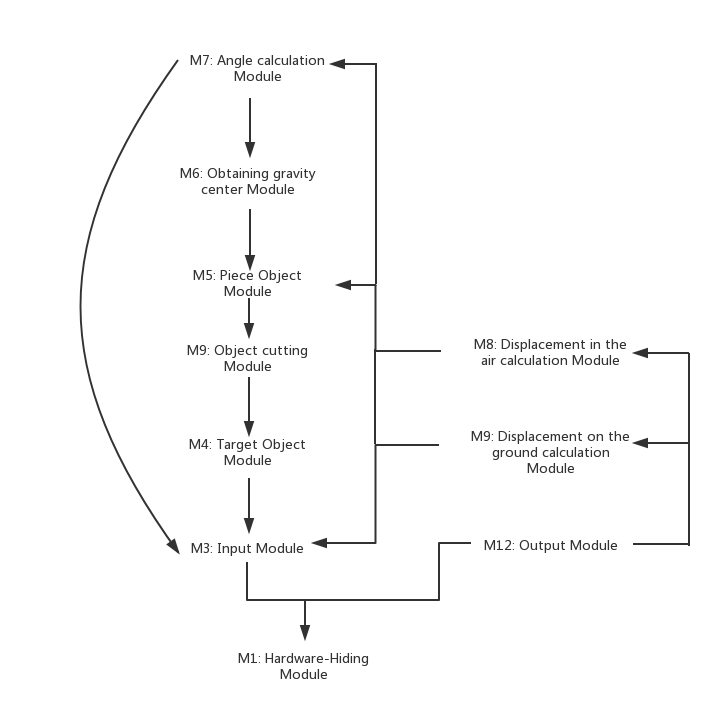
\includegraphics[width=0.7\textwidth]{./Figure1.png}
		\caption{Use hierarchy among modules}
		\label{FigUH}
	\end{figure}
	
	\wss{Was there any thought to having a separate module for coordinating the
		output?  Your gui module is responsible for producing output and coordinating
		the calculations.  Shouldn't there be a graphics driver module in the design
		that is provided by Unity?}\\
	\an{Actually I can but not really for now .. because I don't have separate codes fot a separate graphics driver module. I assume the output module handles the graphics part. I don't have any standard output in console. Only error messages will be shown through console.}
	%\section*{References}
	
	\wss{Good start for the design.  Remember that you may have to modify the design
		as you work through the MIS and gain a deeper understanding of how your
		modules interact.}\\
	\an{Thank you very much for the review and great comments ! And yes I modify the design after work through the MIS.}
	
	\bibliographystyle {plainnat}
	\bibliography {MG}
	
\end{document}
